\XeTeXlinebreaklocale "zh"
\XeTeXlinebreakskip = 0pt plus 1pt

\documentclass{beamer}
\usetheme{Copenhagen}

\usepackage{colortbl}
\usepackage{minted}
\usepackage{xltxtra,fontspec,xunicode,calligra}

\usepackage{graphicx}
\usepackage{float}

\defaultfontfeatures{Mapping=tex-text,Scale=MatchLowercase}
\setmainfont{DejaVu Serif}
\setsansfont{DejaVu Sans}
\setmonofont{DejaVu Sans Mono}
\usepackage[slantfont,boldfont]{xeCJK} % 允许斜体和粗体
\setCJKmainfont{WenQuanYi Zen Hei}
\setCJKsansfont{WenQuanYi Zen Hei}
\setCJKmonofont{WenQuanYi Zen Hei Mono}

\title{Rule-Based Regular Routing Method}
\author{
	周聿浩 \and
	翁家翌
}

\setlength{\parindent}{2em}
%\setlength{\parskip}{0.5em}
 
\AtBeginSection[]
{
	\begin{frame}
		\frametitle{Contents}
		\vspace{-10pt}
		\fontsize{9}{7}
		\tableofcontents[currentsection,currentsubsection,hideothersubsections, sectionstyle=show/shaded]
	\end{frame}
}


\begin{document}
\frame{\titlepage}
\begin{frame}{The Problem}
在一个电路板上,给定一个均匀分布的$n\times n$个内部节点,要求确定电路板的大小,计算各个节点到电路板边界的路径,使得各个路径不相交并且长度之和最短。

\begin{figure}[h]
	\centering
	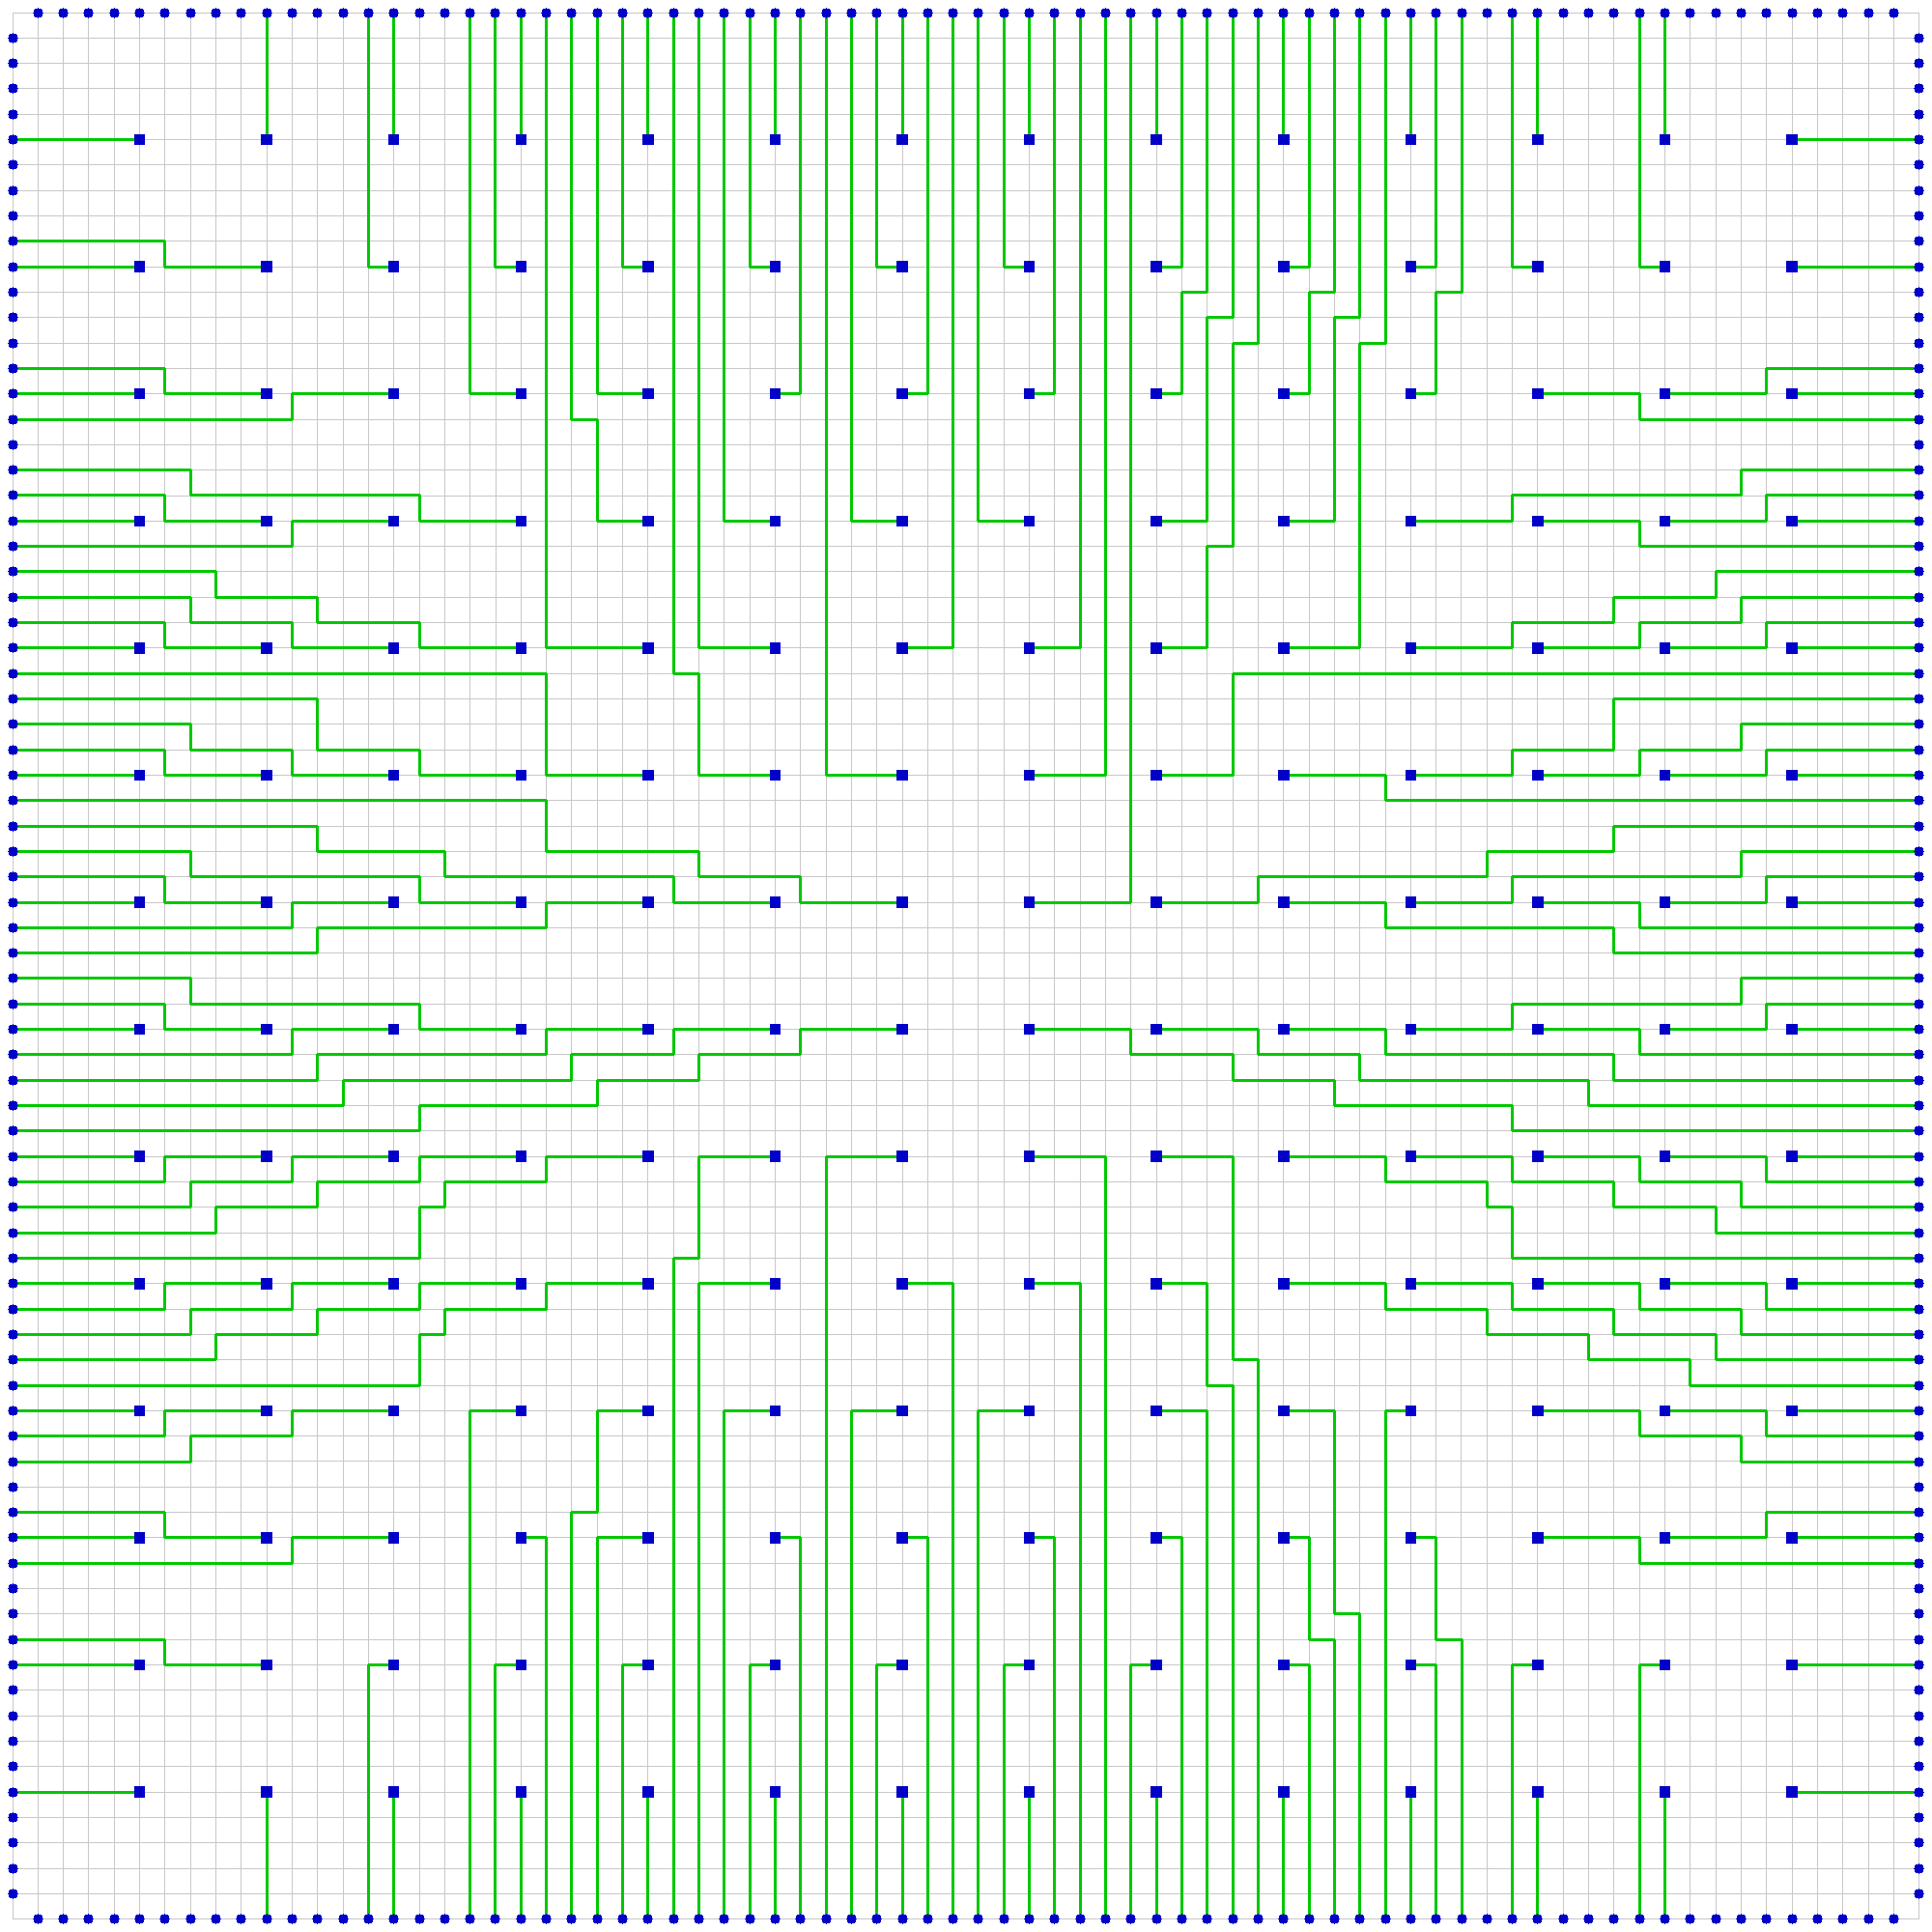
\includegraphics[height=2in]{../project/testcase/small-cases/14x14-76x76.png}
\end{figure}

\end{frame}
\begin{frame}{The Problem}
为了解决这个问题,我们实现了基于费用流的布线方案,该方案能够获得最优解,然而由于不适应与大规模的数据,因此又实现了基于规则的布线方案,该方案可以在可以接受的时间内得到较优的解。

我们支持将计算得到的方案以图片形式输出到文件或窗口,同时也支持以原始路径的形式保存到文件。并且支持从文件中读取原始数据并且显示到窗口。

\end{frame}
\begin{frame}{Some Details}
\begin{itemize}
\item {\bf main.cpp} 主要实现了和用户交互的逻辑
\item {\bf vertex.h} 主要实现了基本的节点类型 Vertex
\item {\bf path.h/cpp} 主要实现了基本的路径类型 Path
\item {\bf route.h/cpp} 整个路径规划算法的抽象接口 Route,同时定义了一些辅助函数用于输出等。
\begin{itemize}
	\item 具体的几个实现。
\end{itemize}
\item {\bf visualization.h/cpp} 用于可视化算法输出
\end{itemize}

\pause
Route 的具体实现都不对用户可见,利用一个工厂函数来创建其实例同时转换为基类的指针。为了减少用户手动删除造成的不必要错误,使用 std::shared\_ptr 来管理内存。

另外,对于读取已经存在的路径数据的类,利用了适配器模式将读取结果保存在Route里。
\end{frame}

\begin{frame}{Algo - MCMF}
题目可以抽象为给定一张图,寻找一些点不相交路径,使得总长度最短。

\pause
每个点只能经过一次?拆点!

\pause
对于每一个节点,由于可以向其相邻节点前进,就让该节点向四周连边。

这样,计算最小费用最大流之后就可以得到最优方案了。

\pause
此外还有一个关于最小电路板大小的问题,可以利用二分答案来进行计算。

这个计算过程中只需要判断合法性而无需最优性,我们可以利用最大流算法而忽略费用以提高速度。
\end{frame}

\begin{frame}{Algo - Rule}
\begin{figure}[htp]
\centering
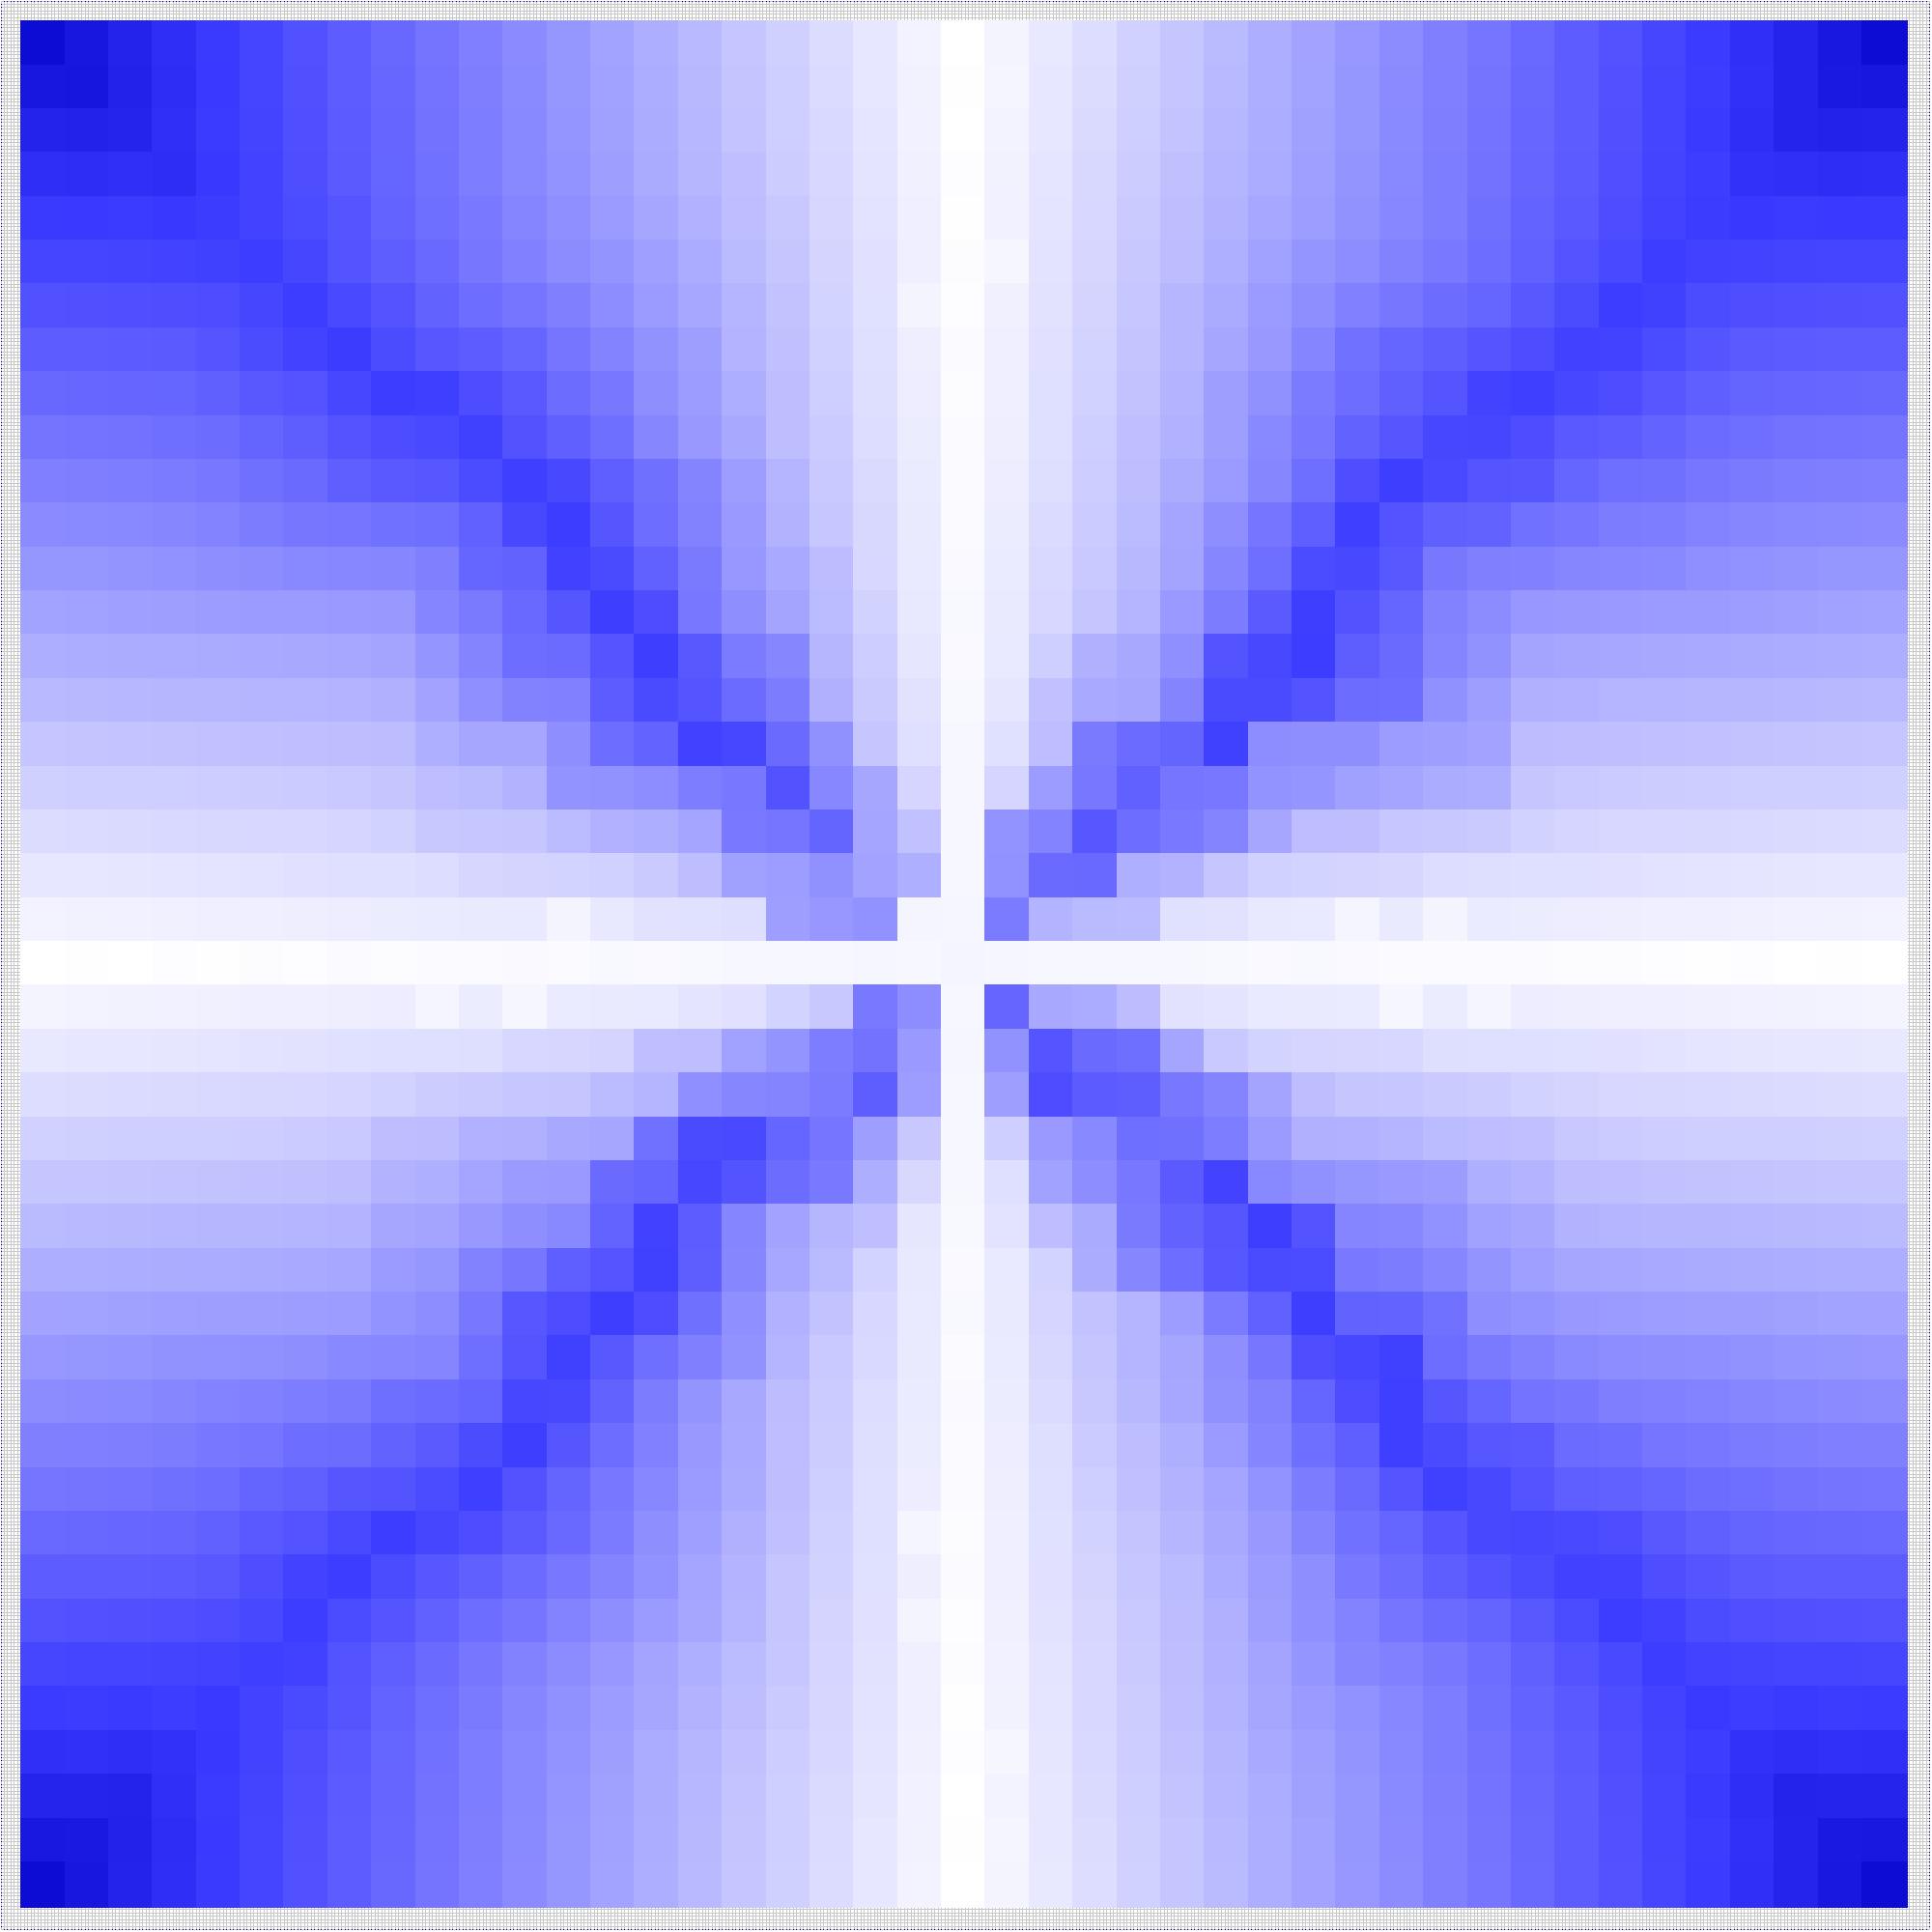
\includegraphics[width=0.5\linewidth]{../project/testcase/label/43.png}
\caption{将费用流得到的布线方法可视化之后……喵喵喵?}
\end{figure}
\end{frame}

\begin{frame}{Algo - Rule}
\begin{figure}[htp]
\centering
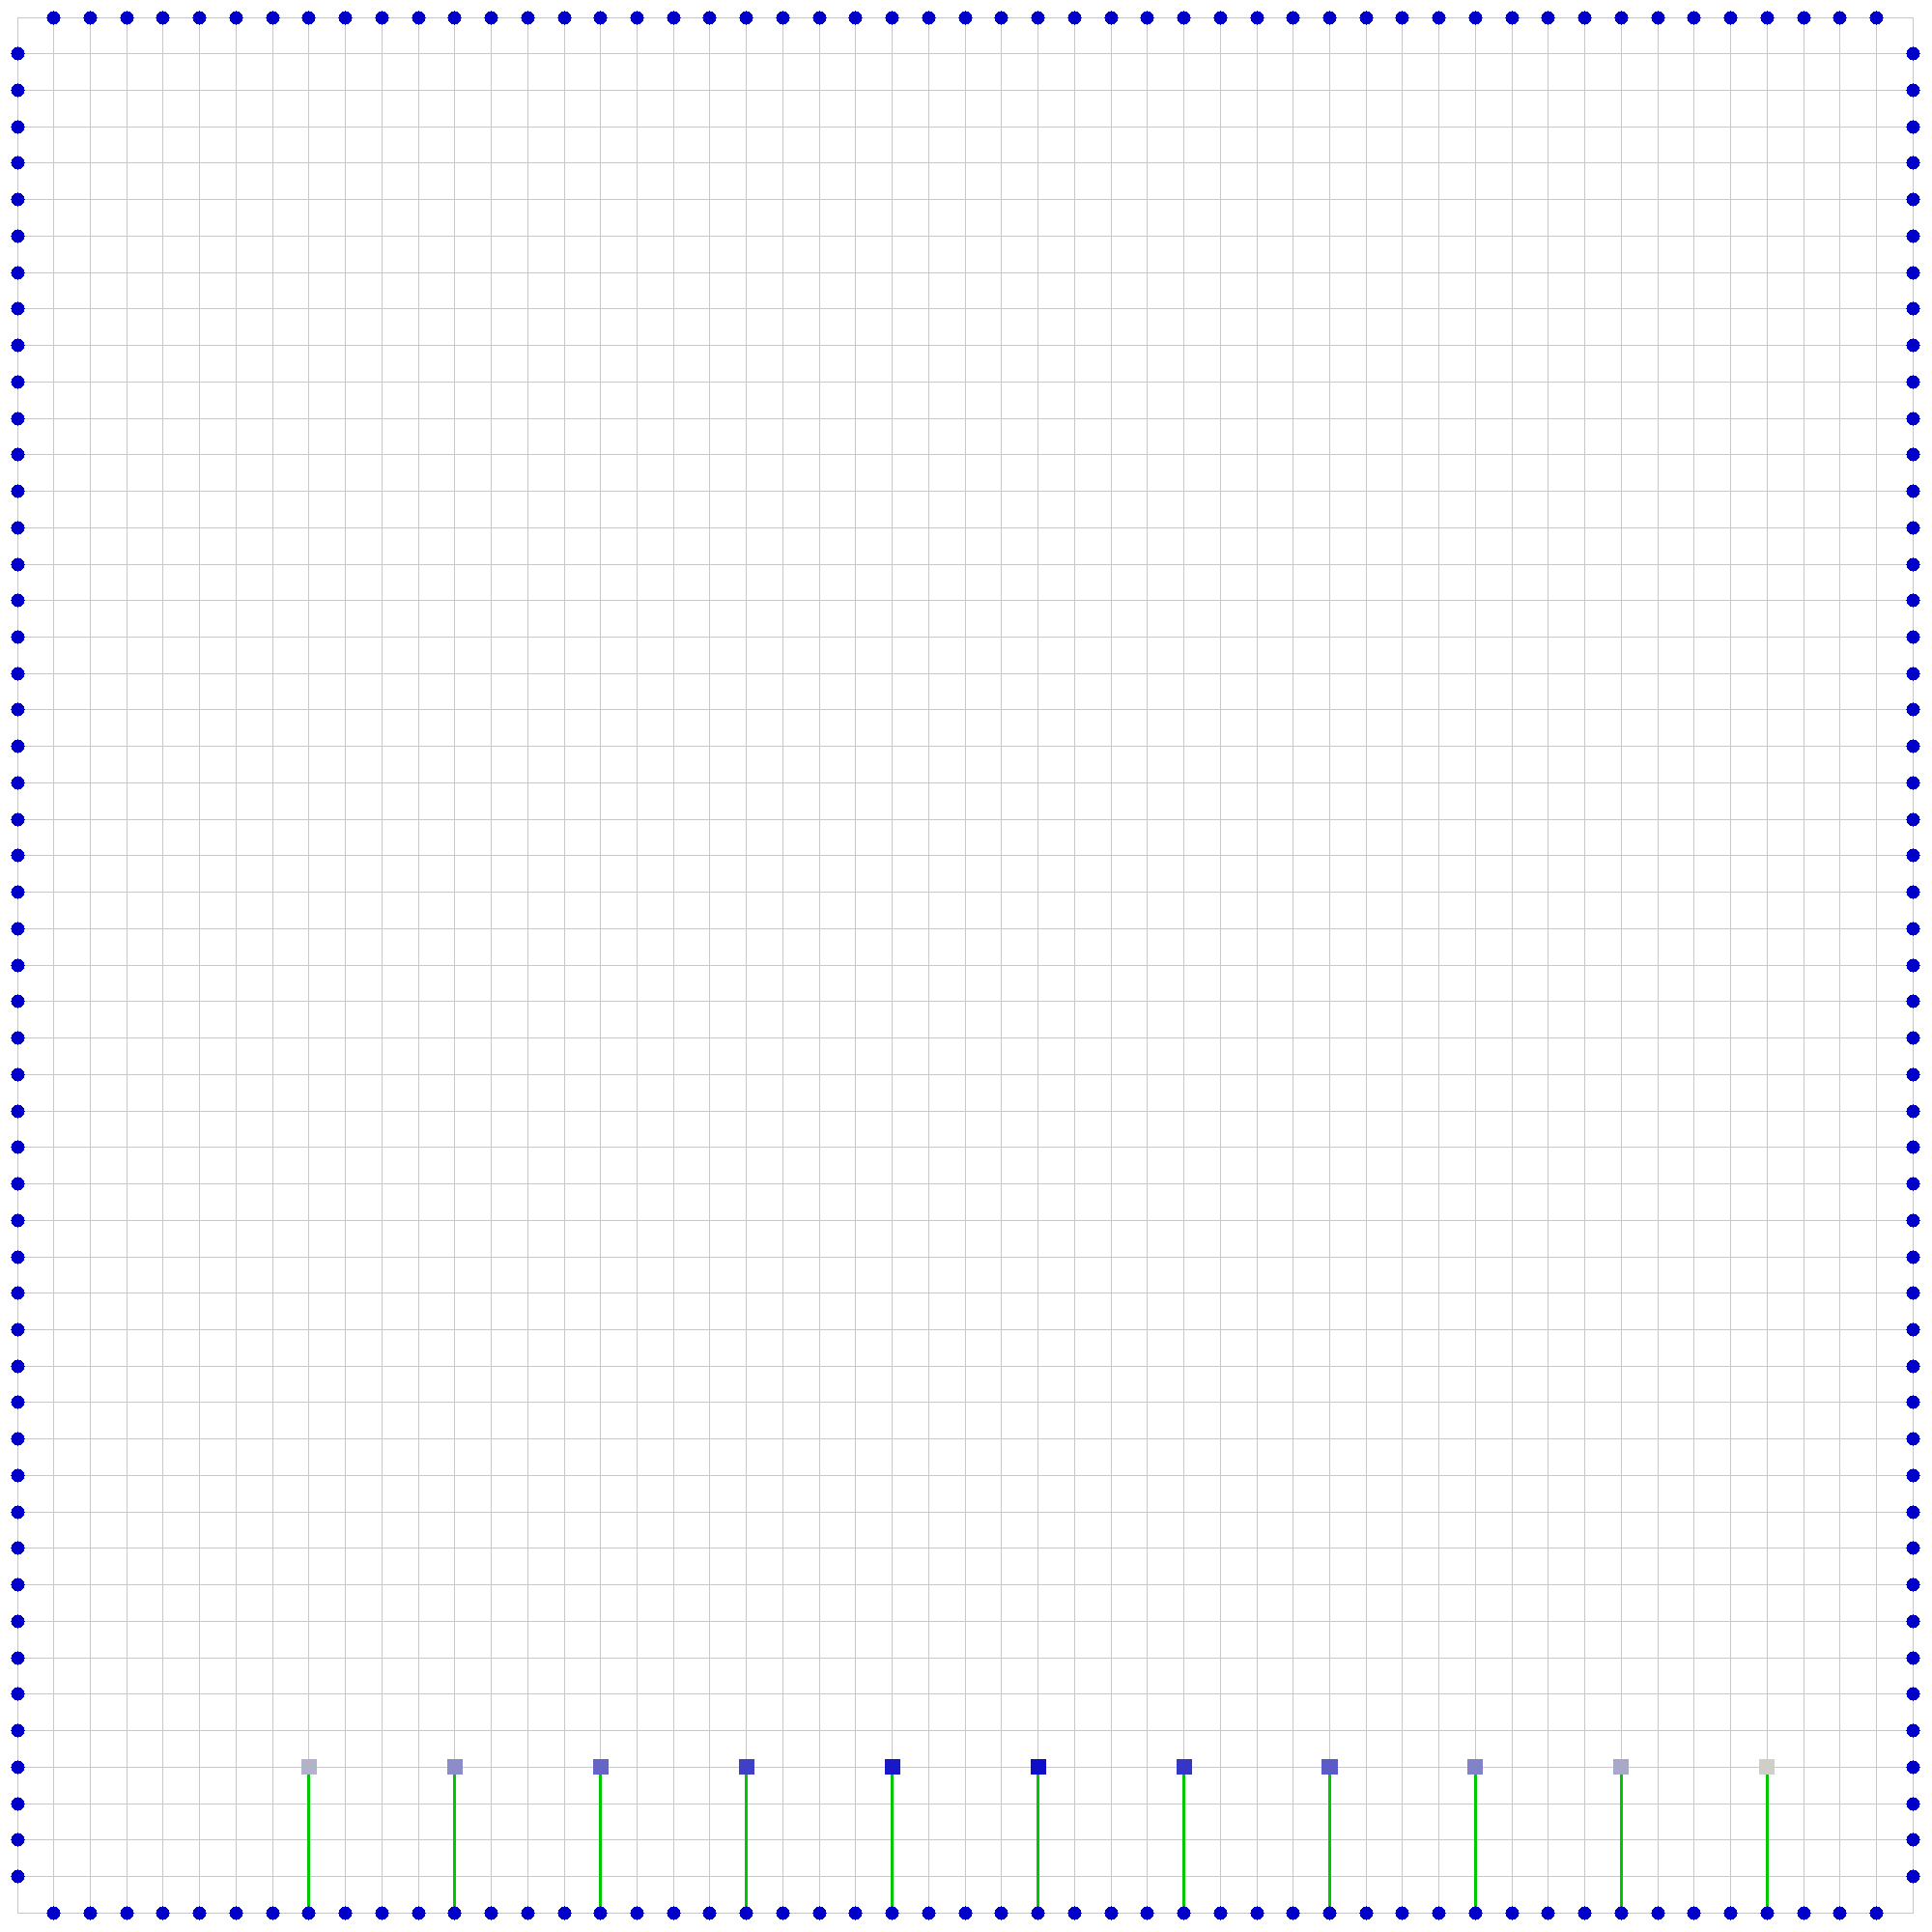
\includegraphics[width=0.25\linewidth]{../project/doc/12_1.png}
~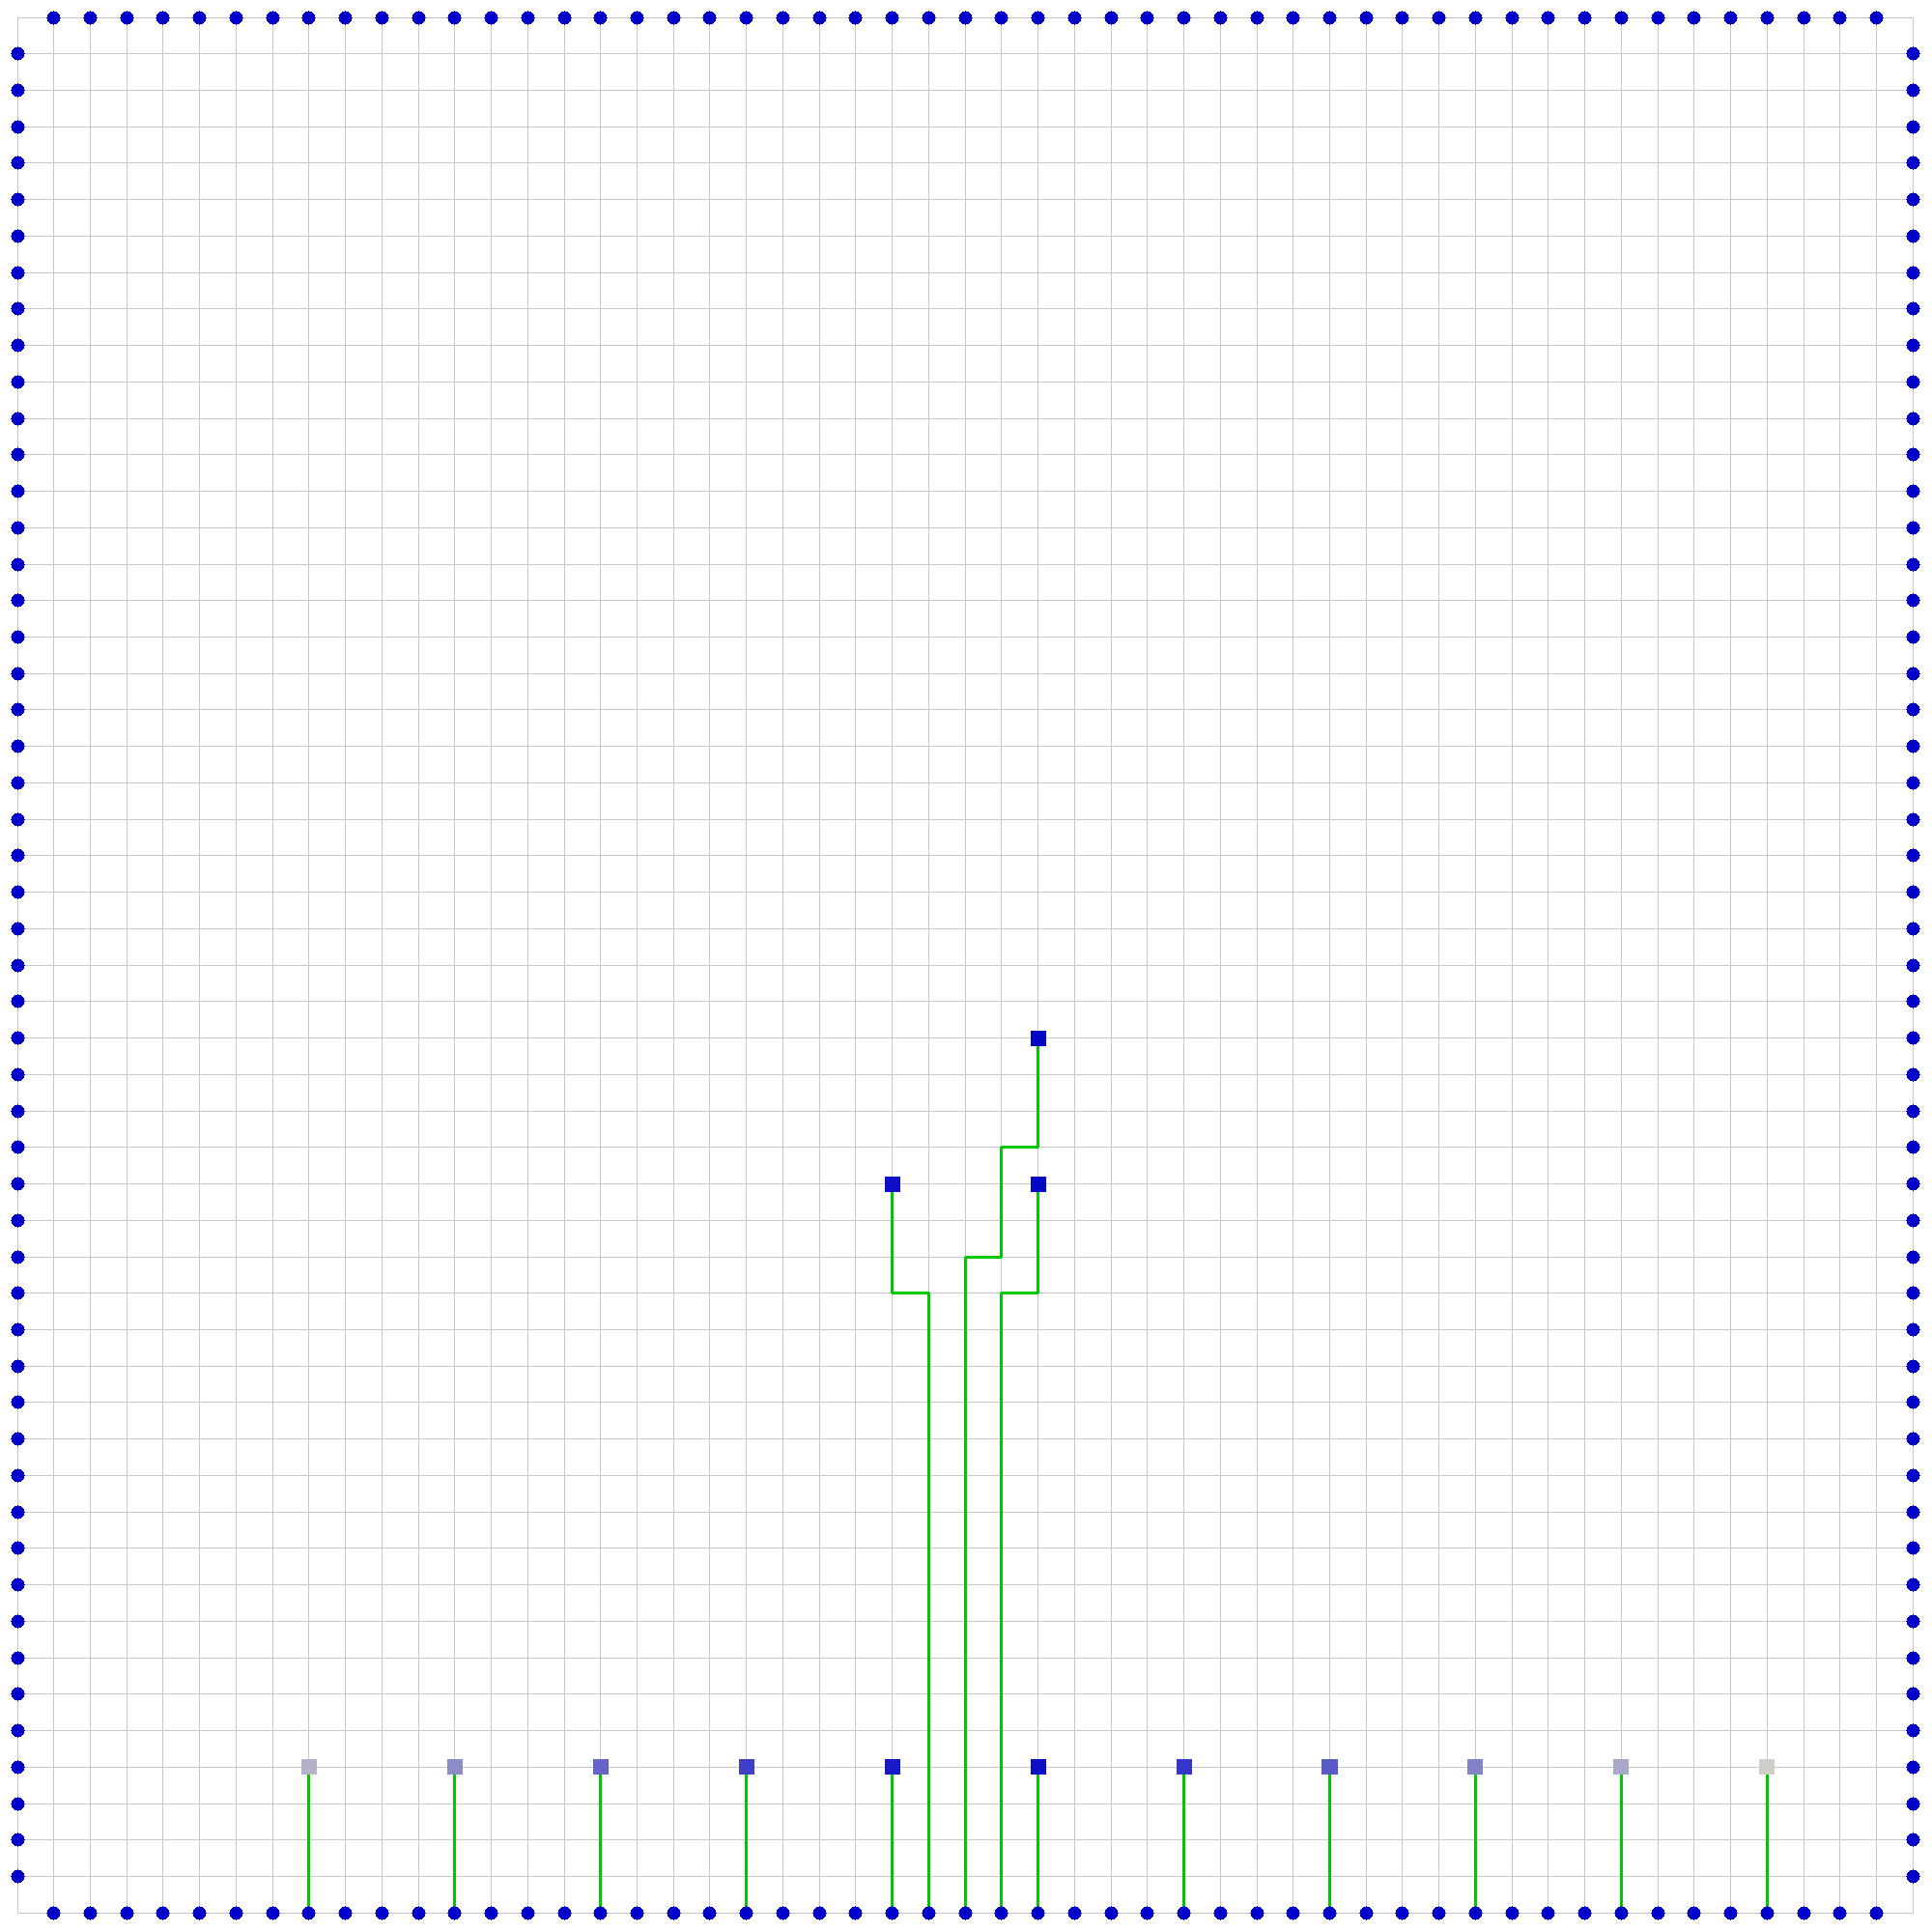
\includegraphics[width=0.25\linewidth]{../project/doc/12_2.png}
~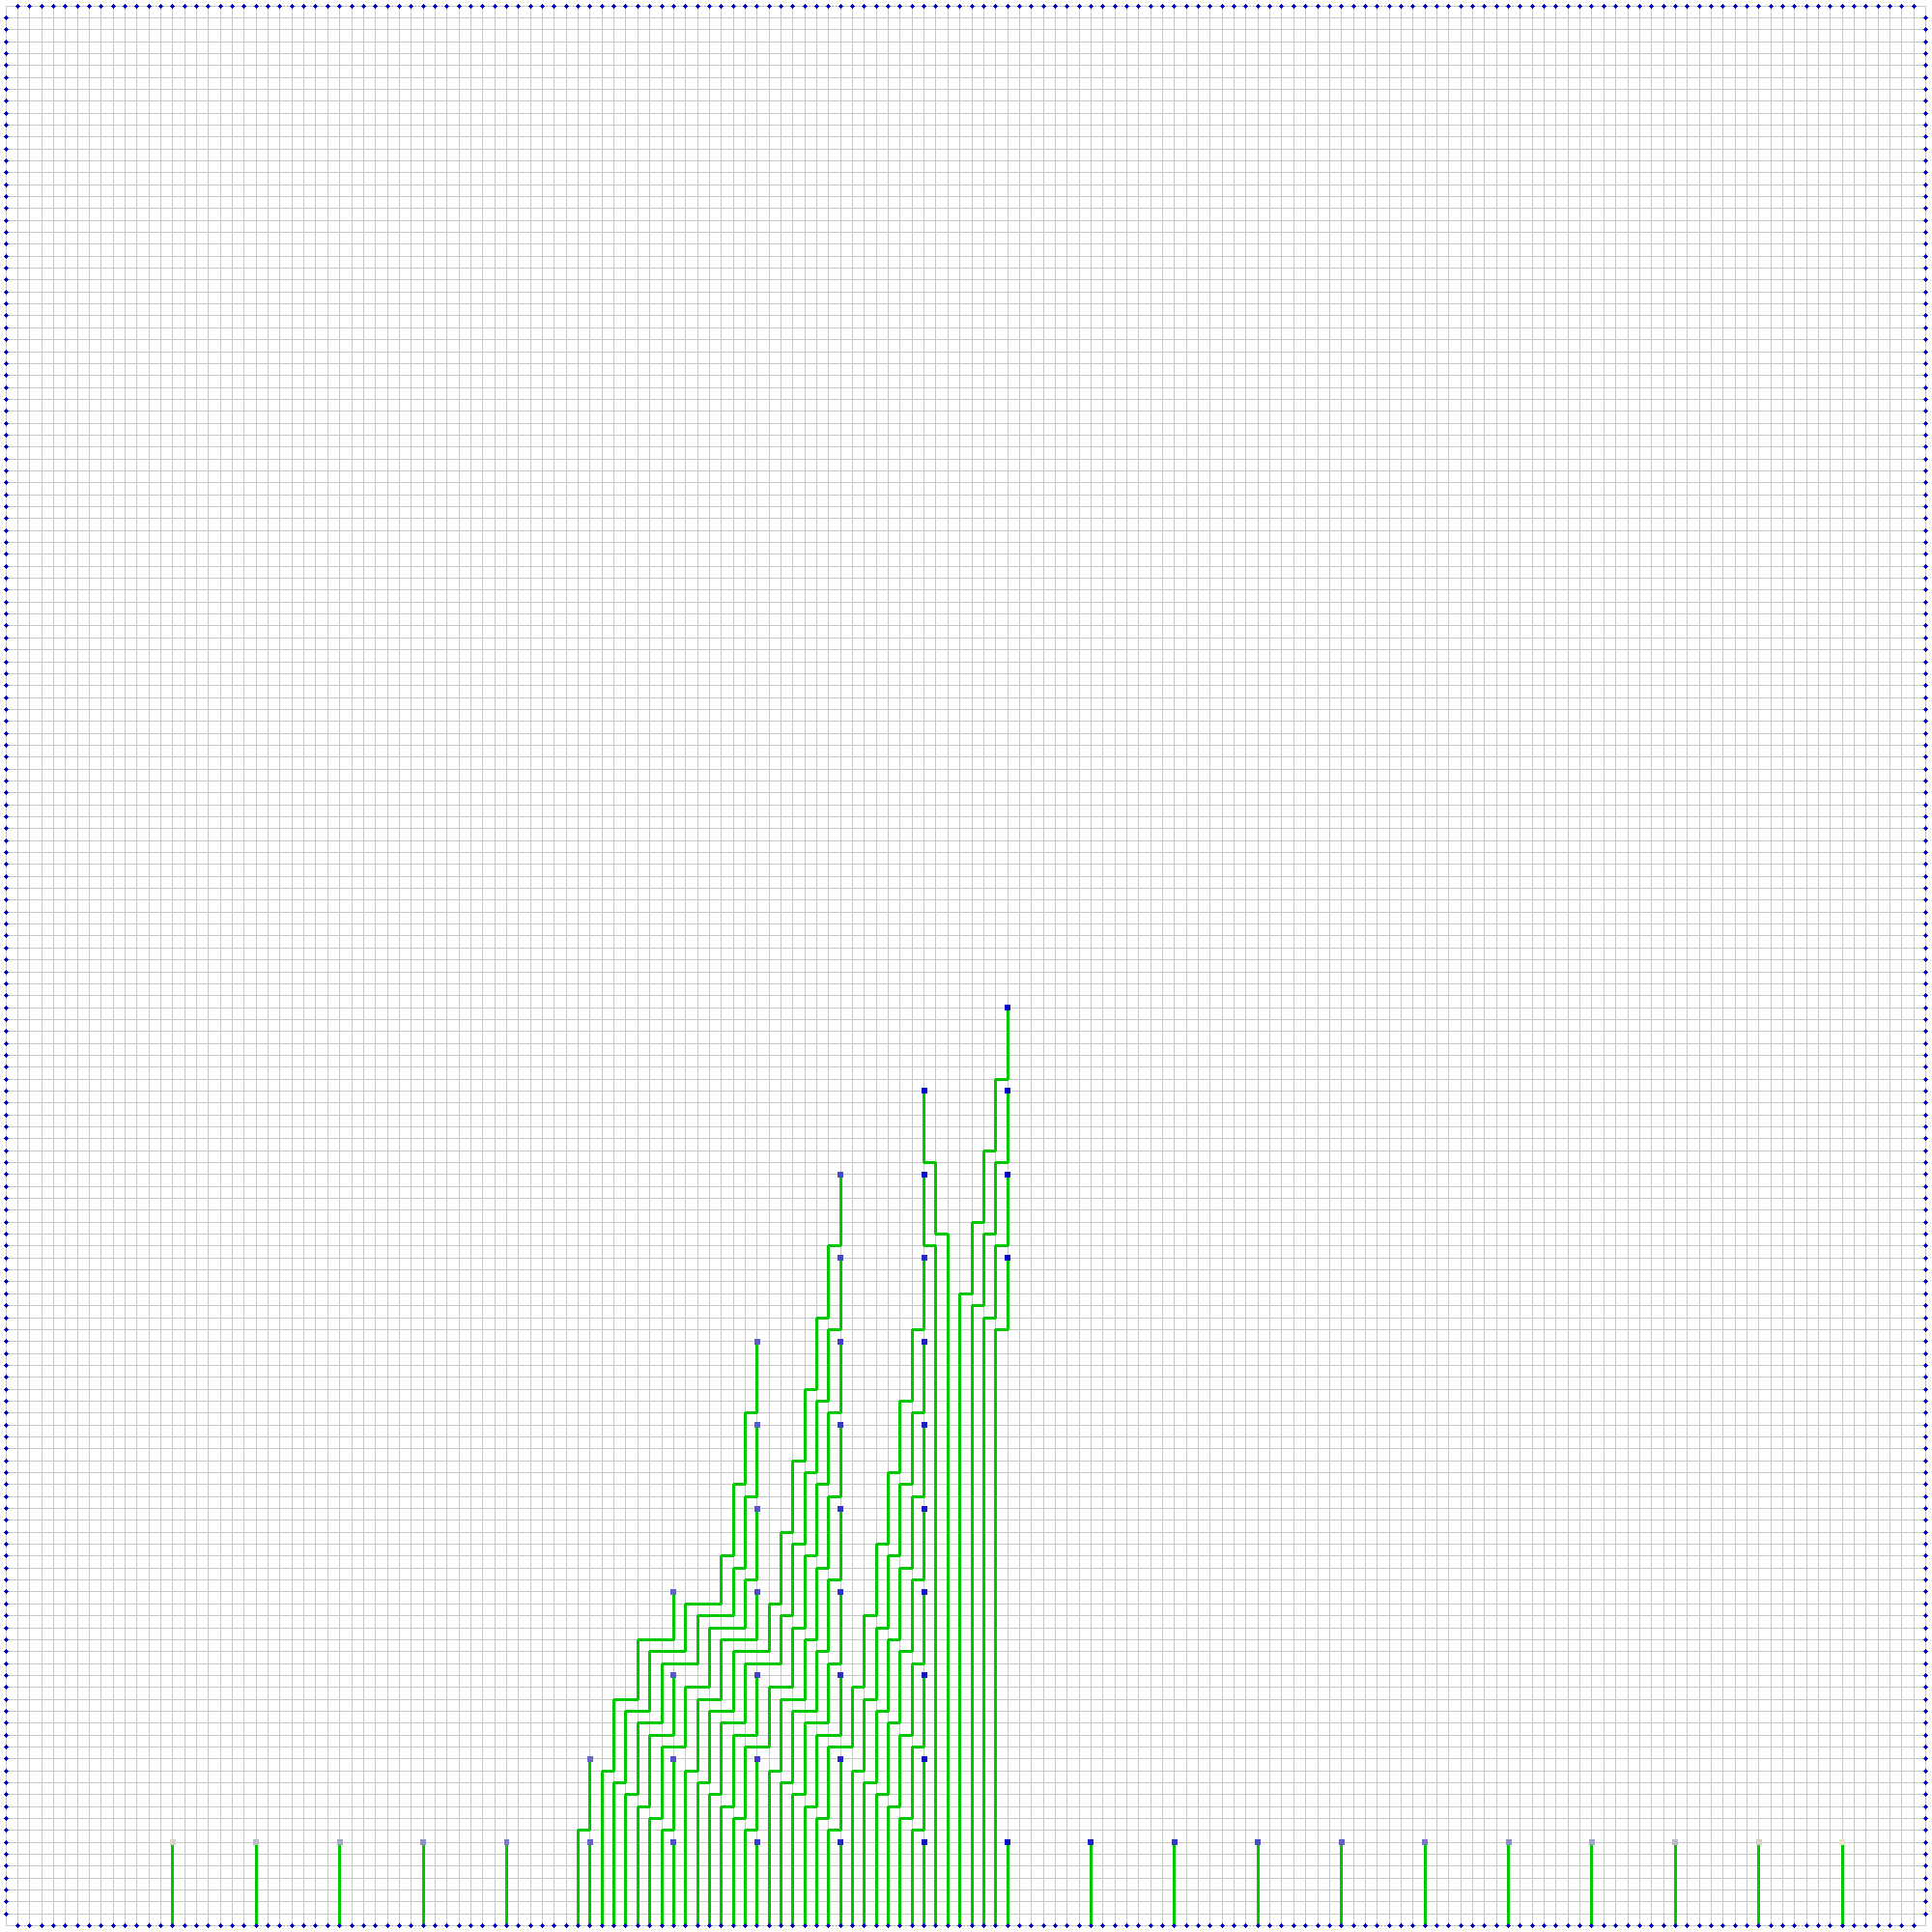
\includegraphics[width=0.25\linewidth]{../project/doc/22_3.png}\\
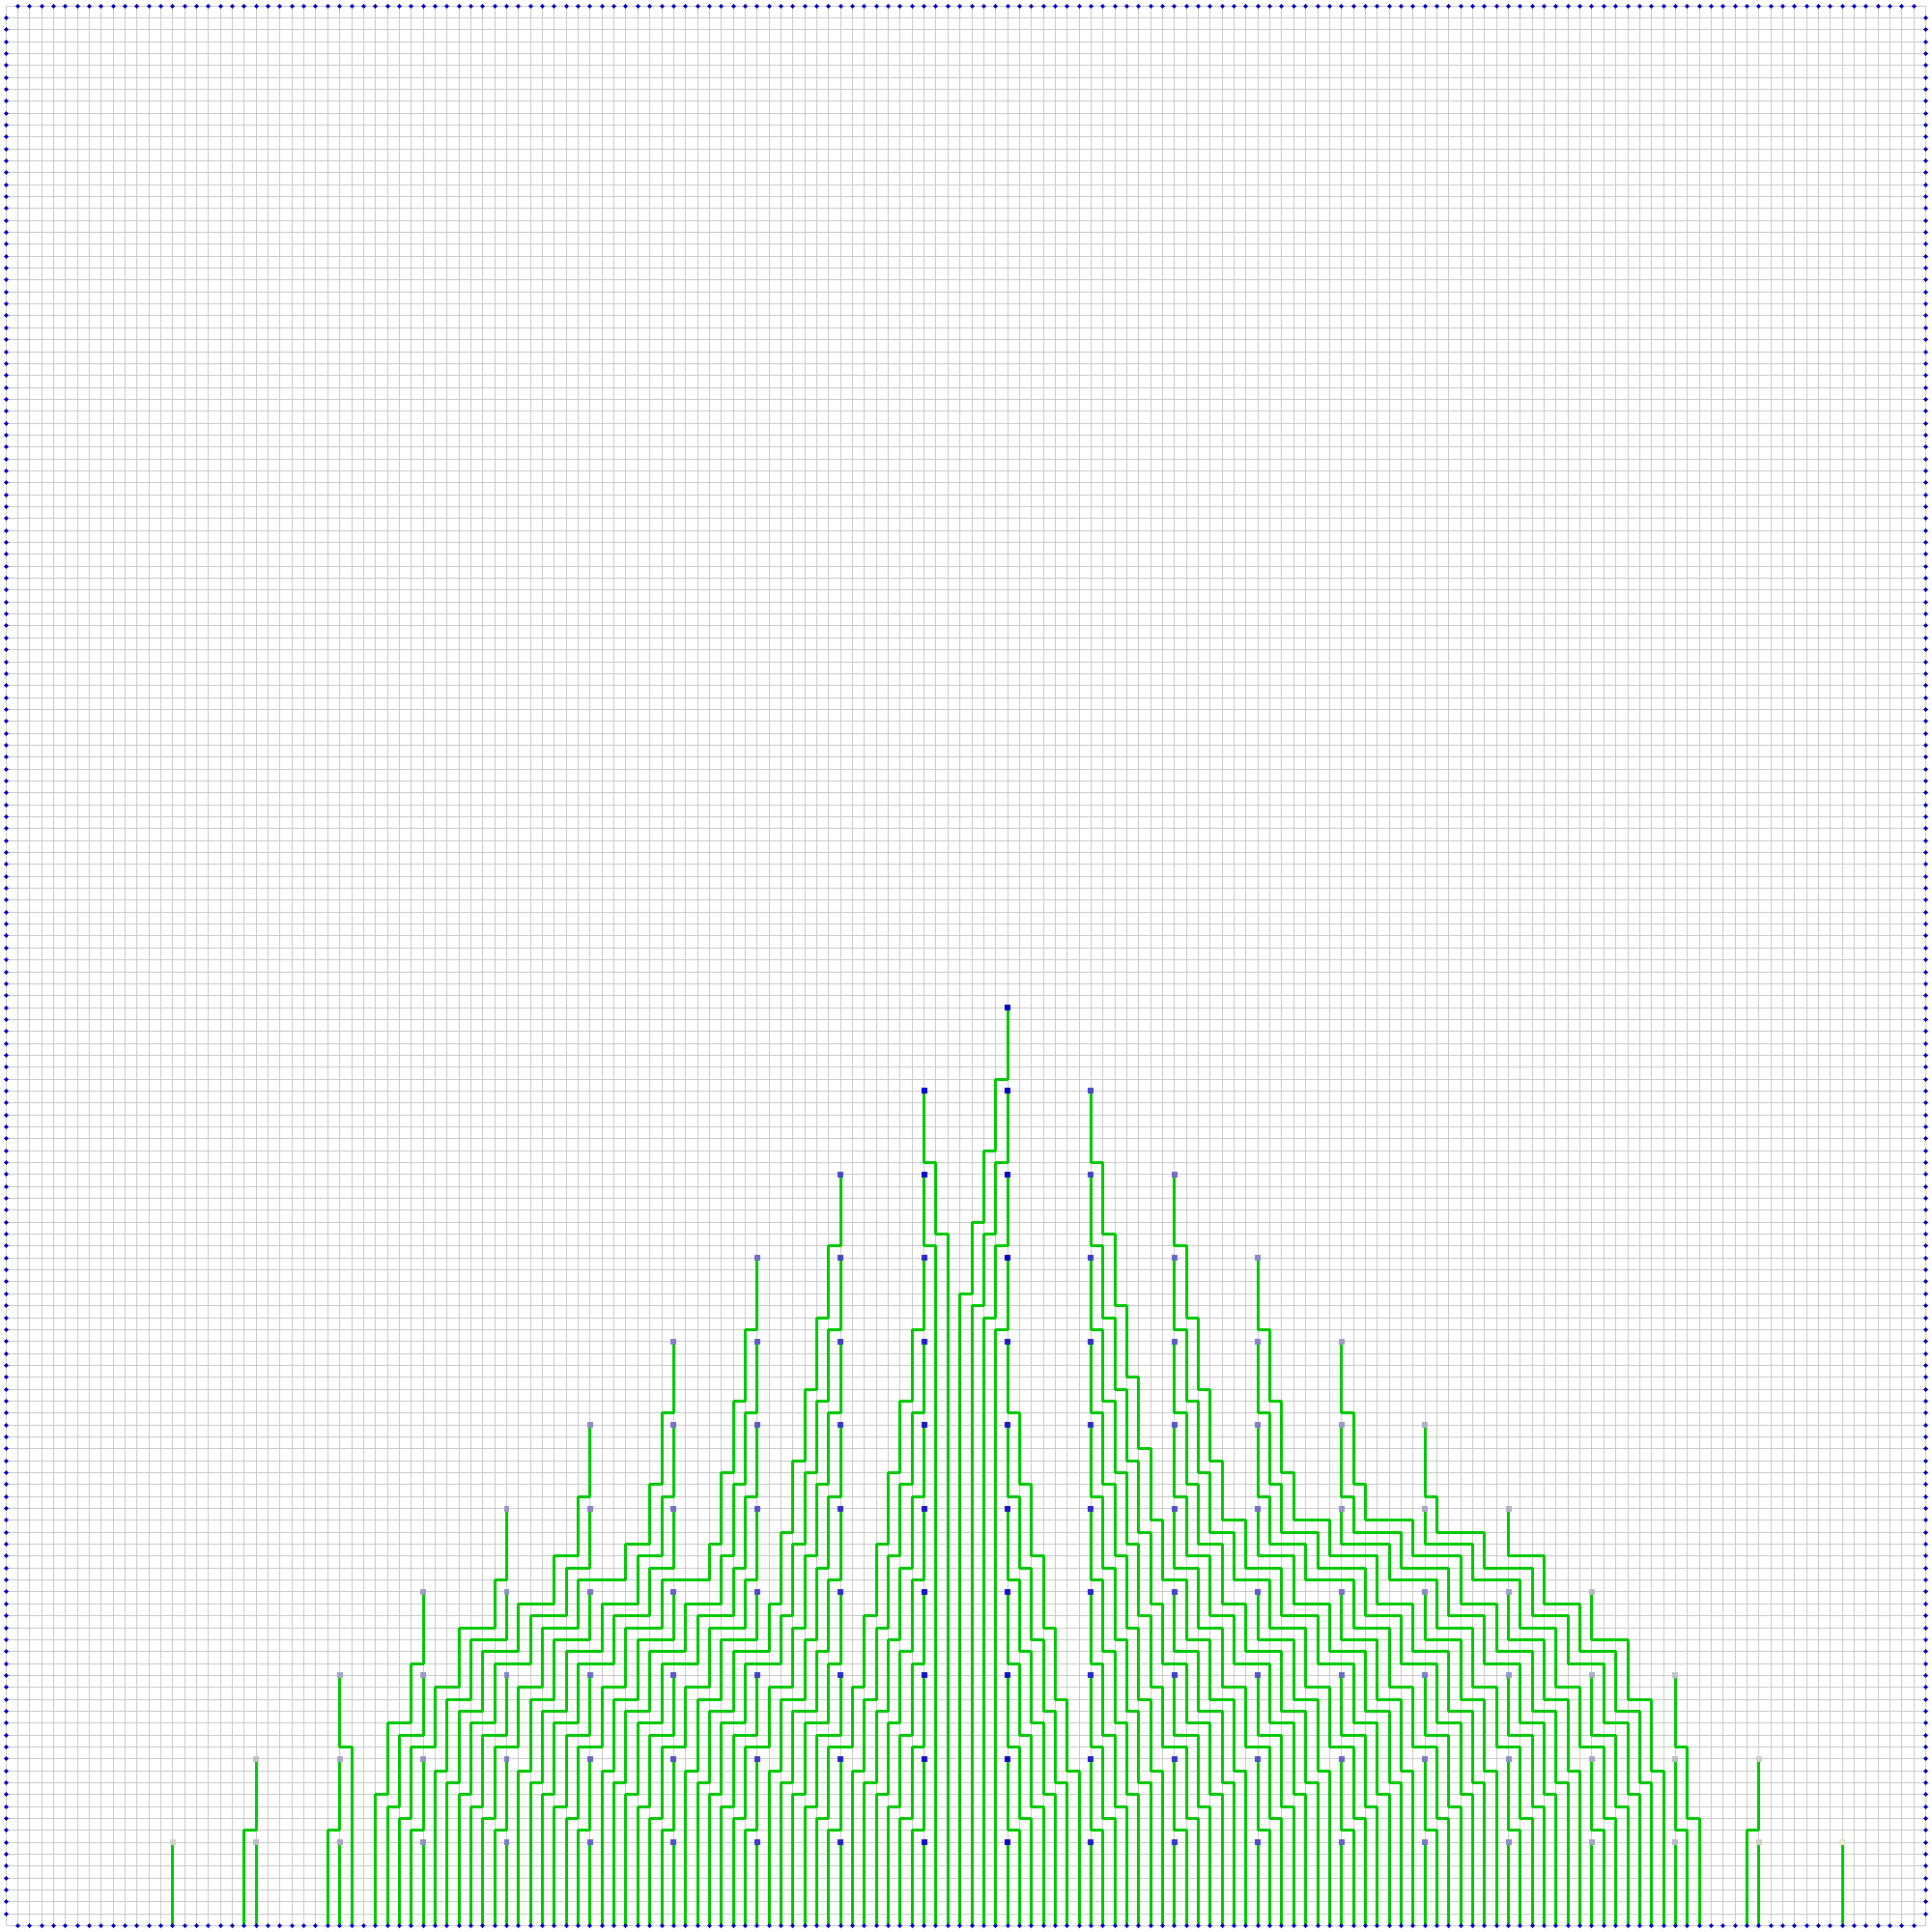
\includegraphics[width=0.25\linewidth]{../project/doc/22_4.png}
~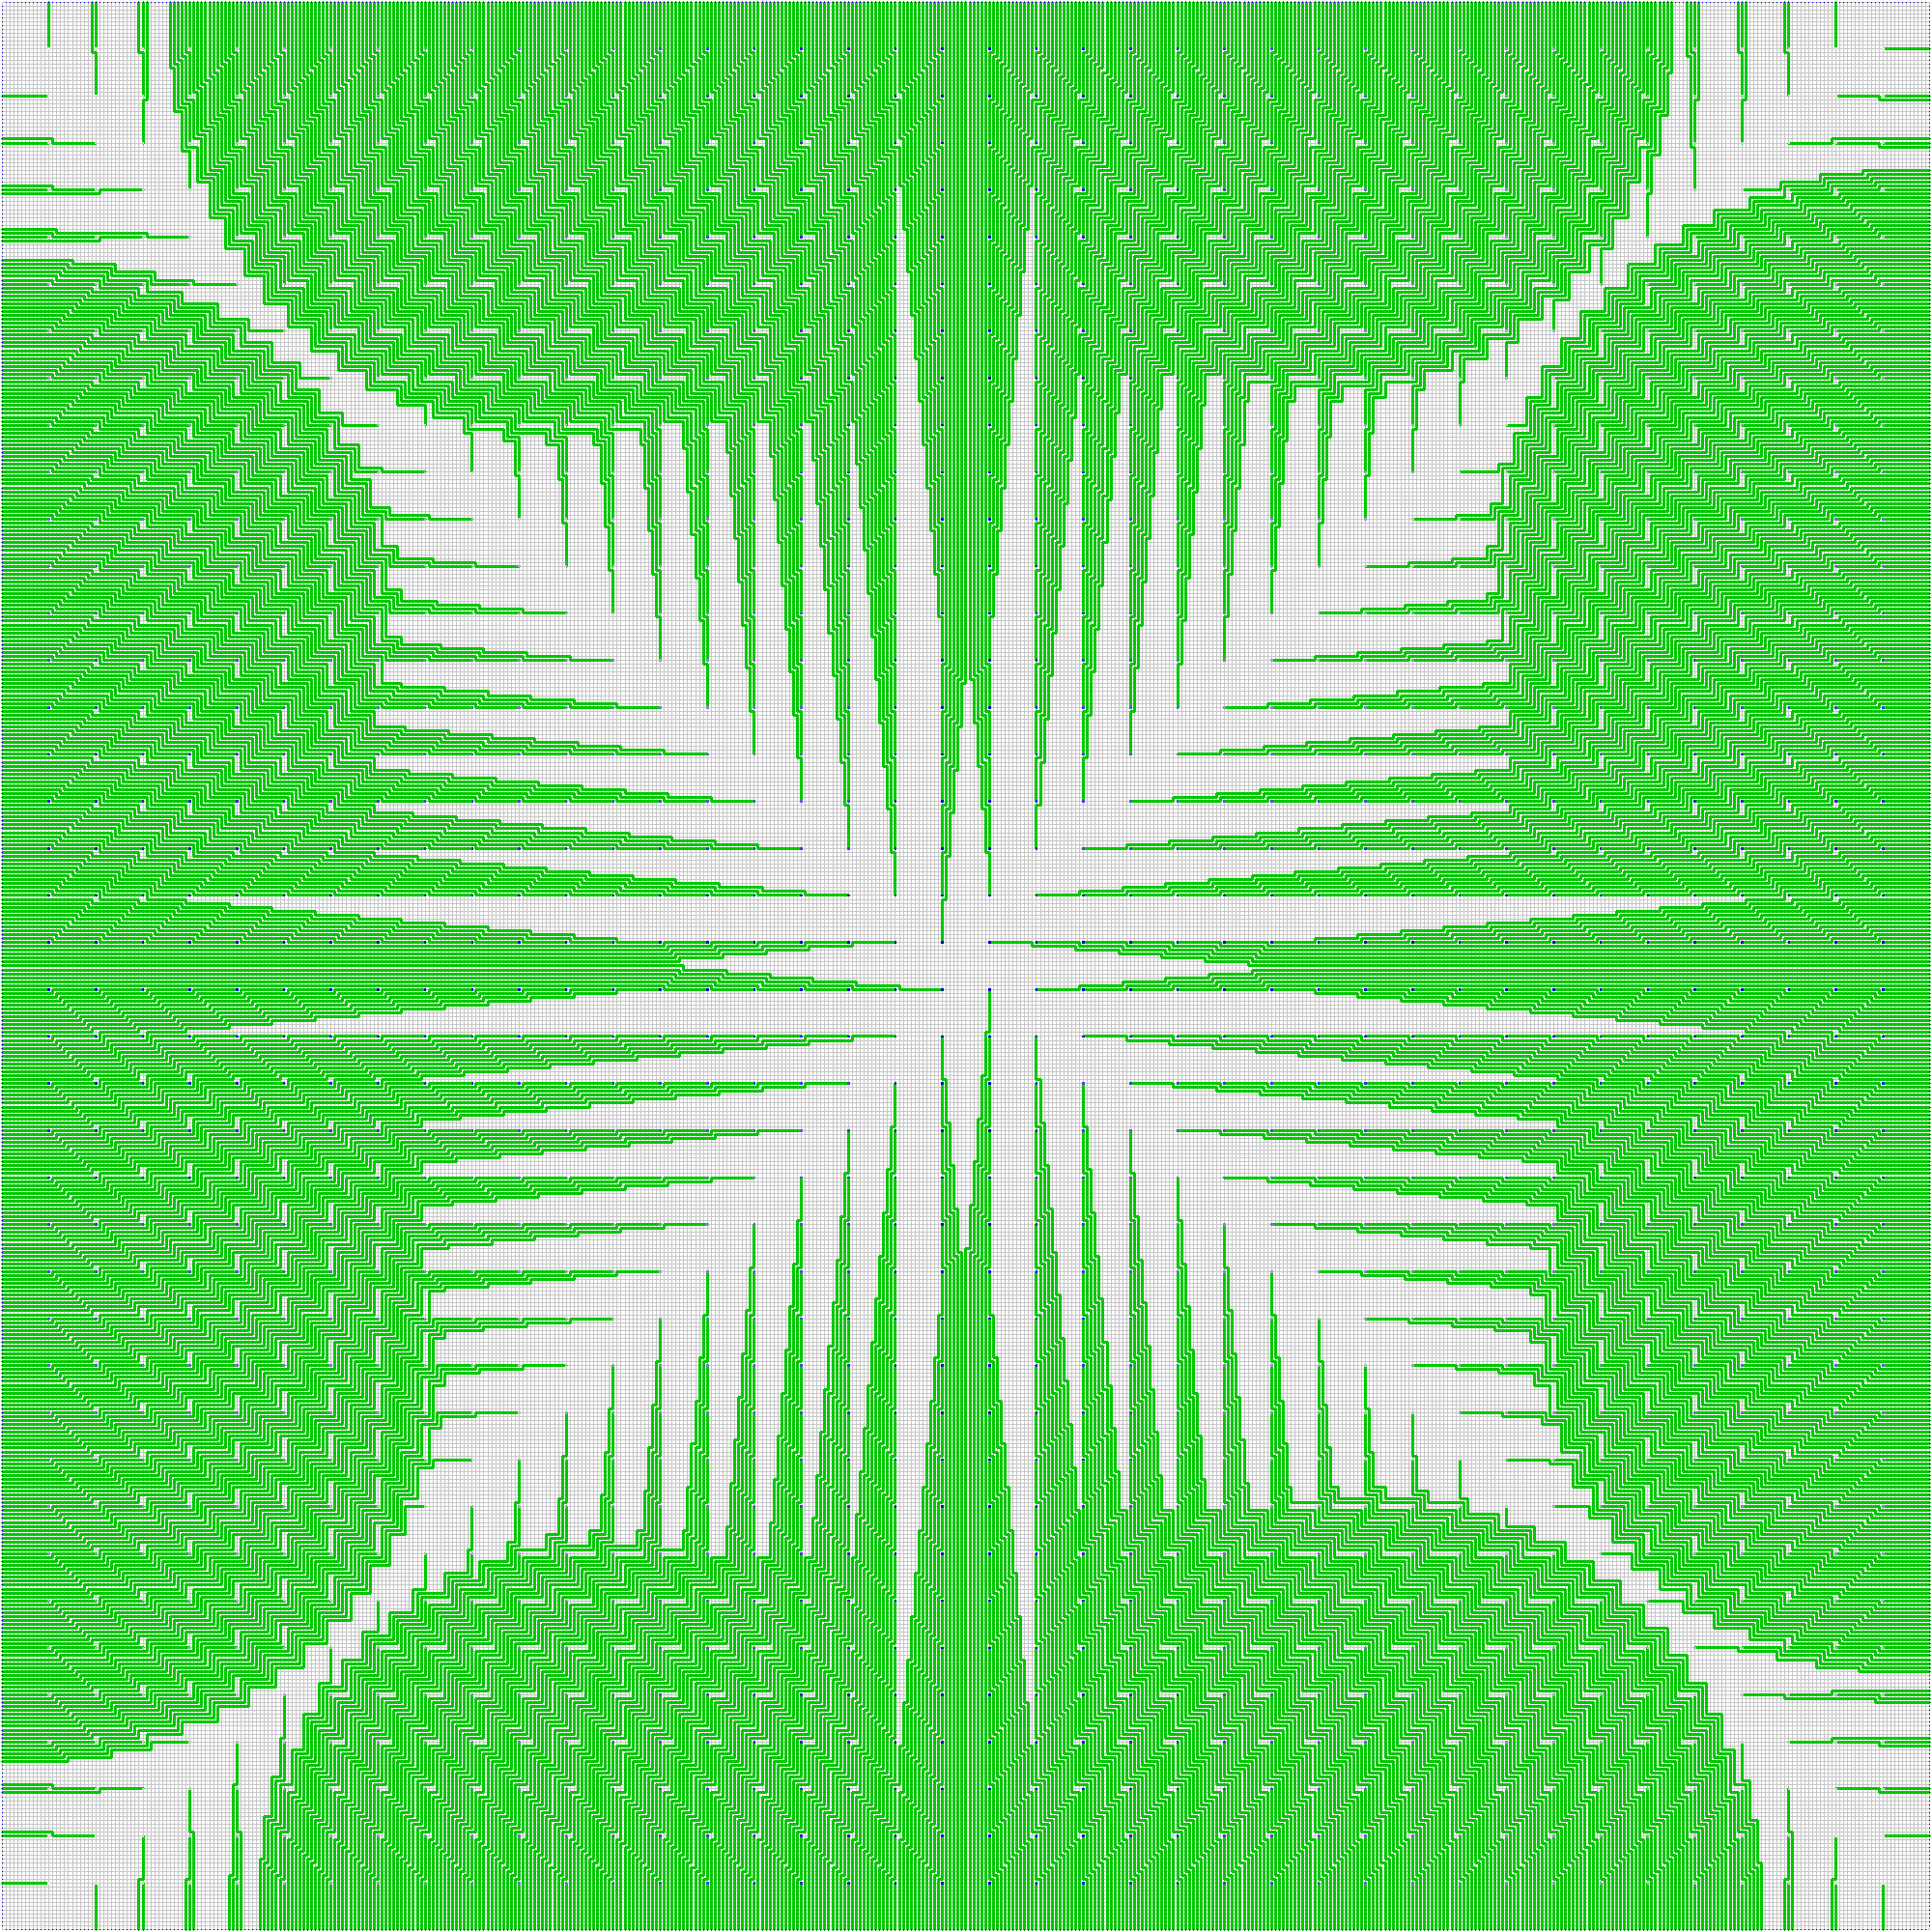
\includegraphics[width=0.25\linewidth]{../pre/40.png}
~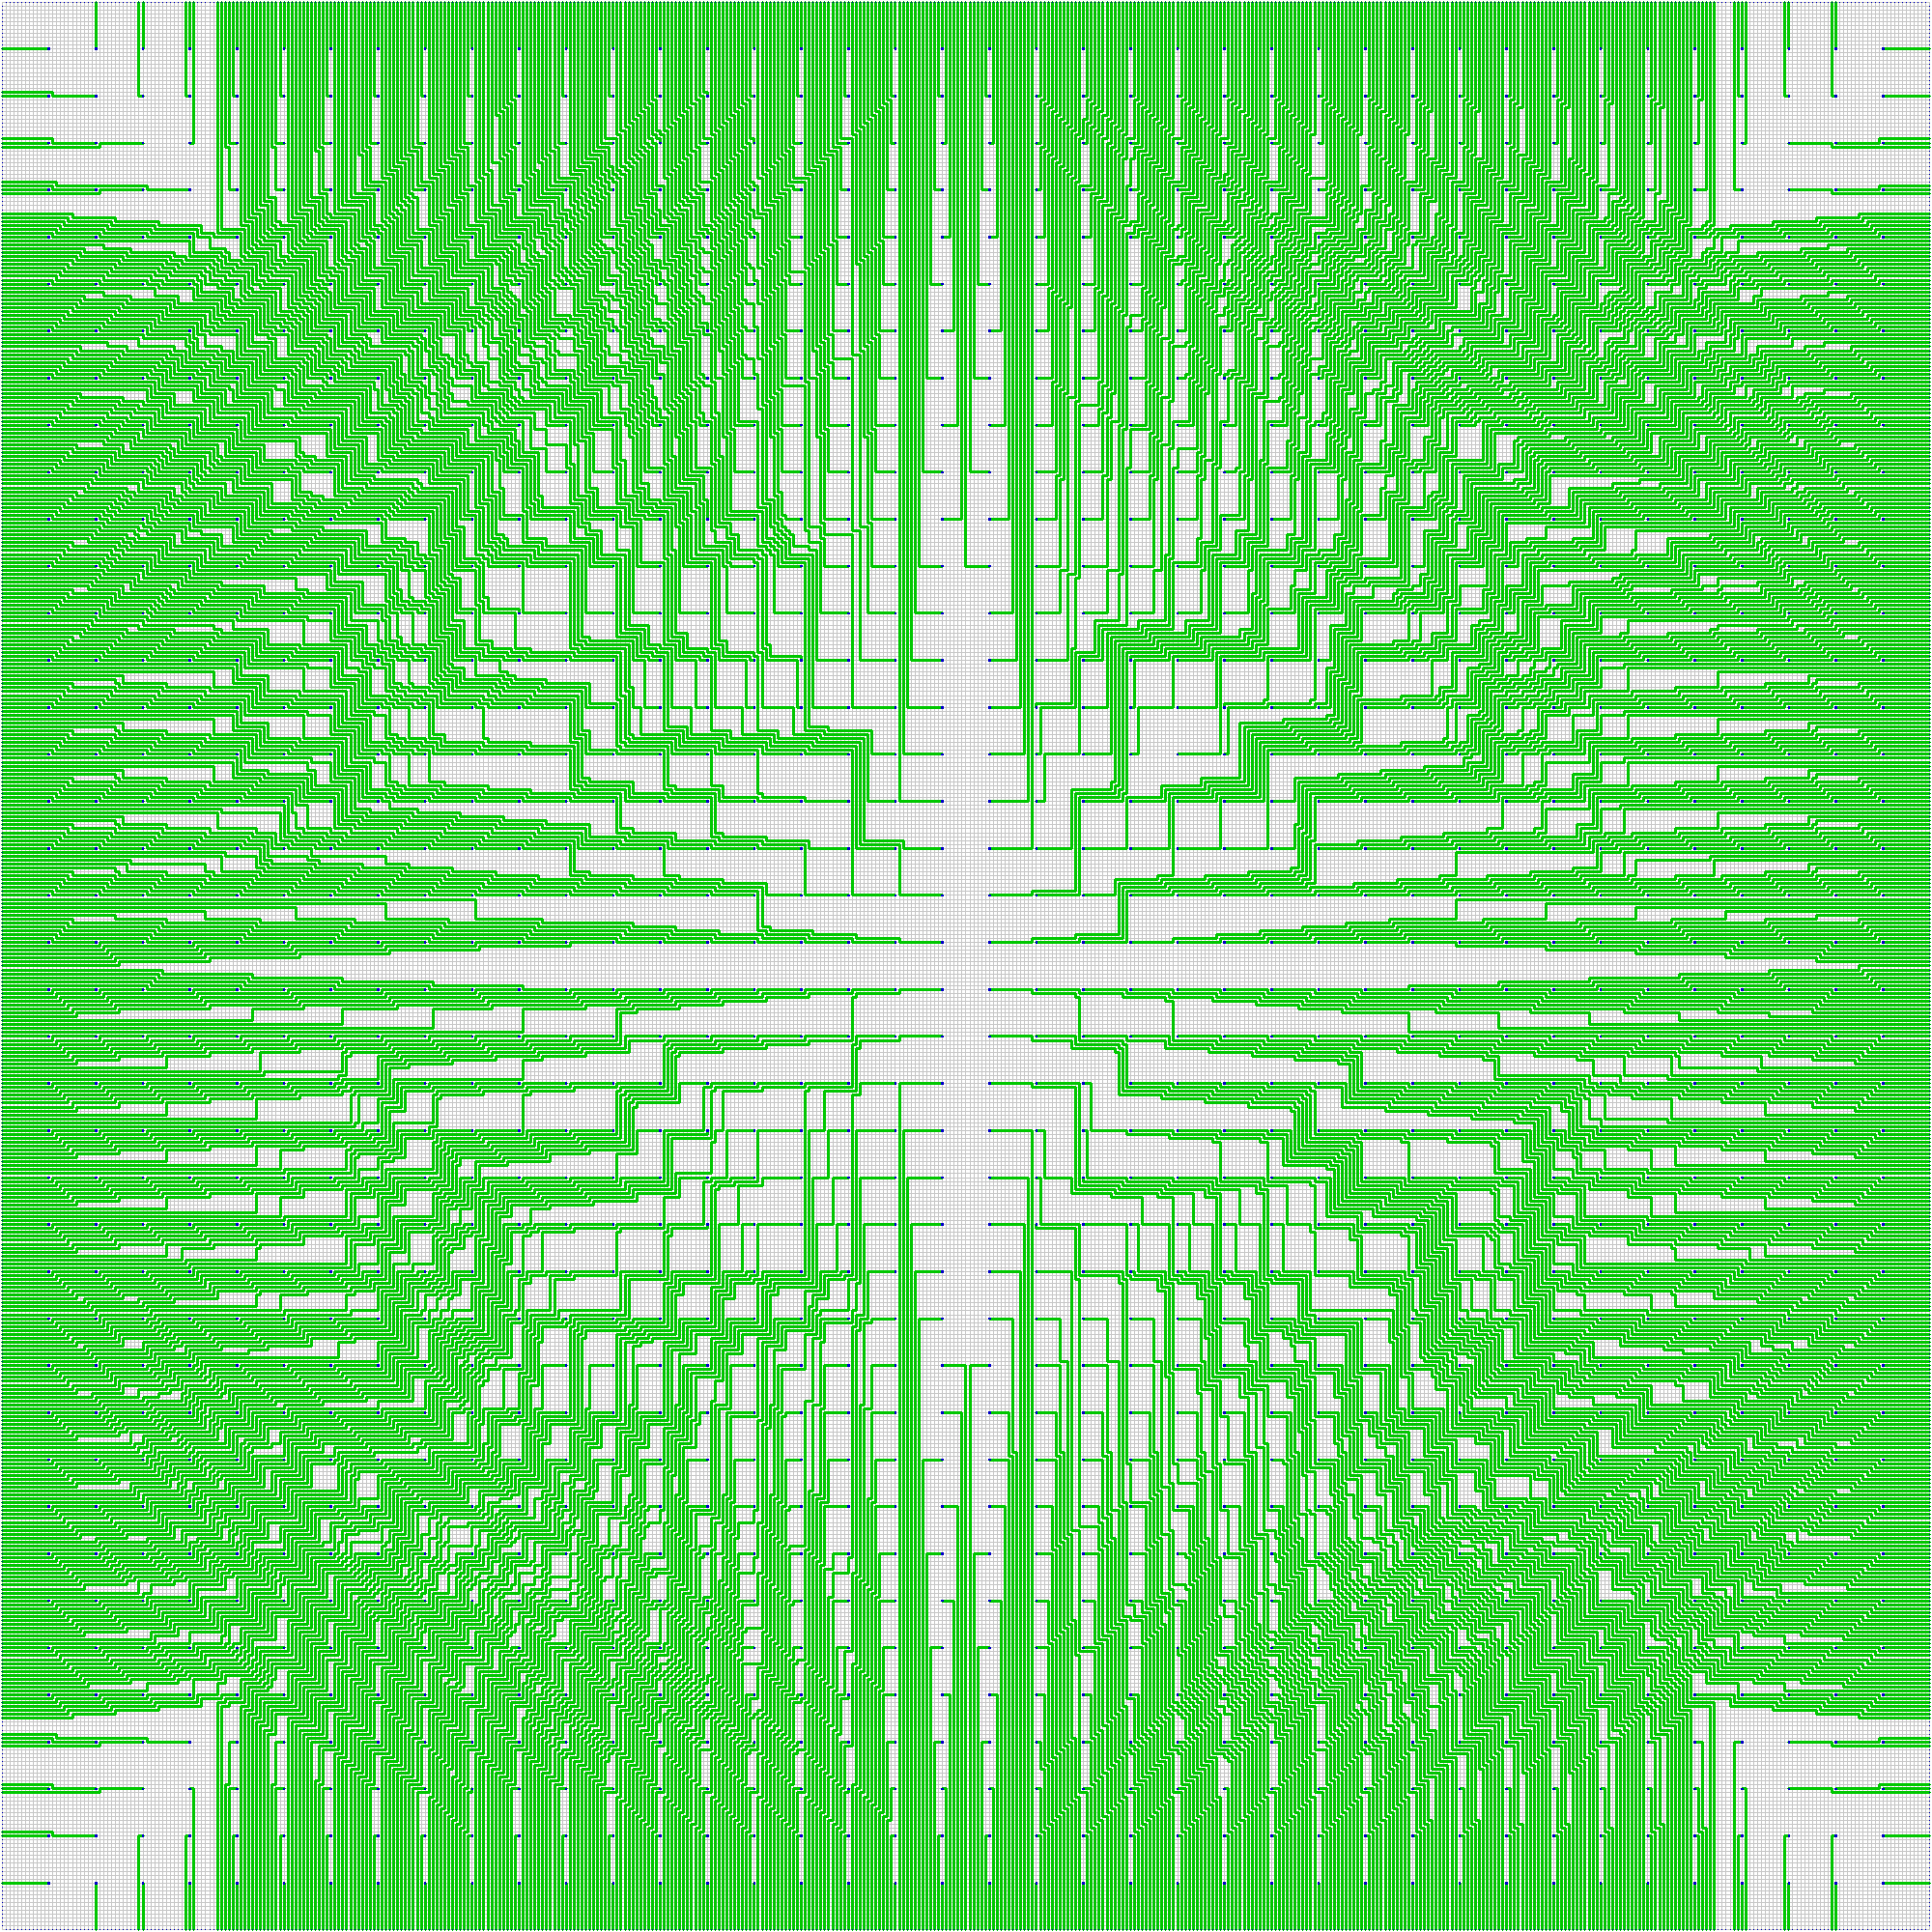
\includegraphics[width=0.25\linewidth]{../project/testcase/small-cases/40x40-493x493.png}
\caption{图解基于规则的布线方法}
\end{figure}
\end{frame}

\begin{frame}{Algo - Rule}
在实现过程中,考虑到$80\times 80$的数据,网格图有$1945\times 1945$的大小,因此寻找路径的算法成为了效率实现的瓶颈。本人使用了$A^*$算法替代传统的BFS算法,估价函数设计成尽量贴着已存在的路径进行寻路,从而实现了效率正比于路径长度的高效算法。

经检验,该算法在$1\sim 80$的数据中只有两个数据需要一些微调,其他数据均快速出解。
\end{frame}

\begin{frame}{Performance}
理论上分析,对于n个点,m条边并且容量都为1的\emph{MCMF},时间复杂度为$O(nm^2)$,而\emph{Dinic}的时间复杂度为$O(\min{(n^{2/3},m^{1/2})}\cdot m)$。在这个问题中,记$n^2$为需要连接的点的个数,$n\in [1,80]$,$N$为电路板的边长,结果表明$\frac{N - 1}{n + 1}\in [\frac{n}{4}, \frac{n}{3}]$,因此可以知道$N = \Theta(n^2)$。

因此复杂度可估计为\emph{MCMF}:$O(n^6)$,\emph{Dinic}:$O(n^3)$。

而人工设计的基于规则布线的方法几乎是正比于布线的总长度,因此时间复杂度为$O(n^2)$。

~\\

\pause 演示一下
\end{frame}
\begin{frame}{Performance}
\begin{table}[H]
\label{tab:1}
\centering
\begin{tabular}{|c|c|c|c|}
\hline
\emph{n} & \emph{MCMF} & \emph{Dinic} & \emph{Rule}\\
\hline
5 & 0.040& 0.040& 0.040\\
\hline
15 & 0.308&0.056 & 0.040\\
\hline
25 & 7.504& 0.404& 0.064\\
\hline
35 &3'25'' & 2.276& 0.148\\
\hline
45 &24'4'' & 14.656& 0.272\\
\hline
55 &数小时 &66.584 & 0.484\\
\hline
65 &数小时 &7'13'' & 0.904\\
\hline
75 &约$8\sim 9h$&约$1h$  & 1.712\\
\hline
\end{tabular}
\caption{性能测试,时间若未注明则以秒计}
\end{table} 
\pause 听说消圈算法巨慢无比?
\end{frame}
\begin{frame}{Performance}
\begin{table}[H]
\label{tab:2}
\centering
\begin{tabular}{|c|c|c|c|c|c|}
\hline
\emph{n} & \emph{MCMF} & \emph{Dinic} & \emph{Rule} & $\frac{Rule-MCMF}{MCMF}\%$&$\frac{Dinic-MCMF}{MCMF}\%$\\
\hline
5 & 79 & 79 & 79 & 0.000&0.000 \\
\hline
15 & 3862&3910&3879&0.440&1.243 \\
\hline
25 & 27394	&   27566	 &  27460	&0.241& 0.628\\
\hline
35 &101775	&  102051	&  101920	&	0.142&0.271\\
\hline
45 & 273183	 & 273811	&  273433	&	0.092 &0.230\\
\hline
55 & 602856	 & 603975	&  603241	&0.064 &0.186\\
\hline
65 & 1167116	& 1168932	& 1167662	&	0.047&0.156\\
\hline
75 & 2057345	& 2060192	& 2058082	&	0.036&0.138\\
\hline
\end{tabular}
\caption{效果分析}
\end{table}
\end{frame}
\begin{frame}{~}
	\begin{center}
		{\Huge\calligra Thank you!}
	\end{center}
\end{frame}
\end{document}
